%!TEX root = ../_thesis.tex
\chapter{Conclusion and Discussion} % (fold)
\label{c-conclusion}
% Resumen resultados itemizados

During this work, we have explored from distinct approaches the sequentiallity in the neuronal dynamics, from the activation of ionic channels to cycle-by-cycle dynamics in CPG circuits. Here is a summary of the main results presented in this thesis:

\begin{itemize}
	\item Importance of the study of sequential dynamics
	\item Universality of sequential dynamical invariants: We explore the dynamical invariants reported in \textit{Lymnaea stagnalis} CPG from experimental and modeling data in a different animal model from the original work. 
	\item The variability distribution in the feeding CPG changes as the neuron stimulated in the model simulation changes.
	\item It is possible to reproduce experimentally the findings of the sequential dynamical invariants observed in the computational model simulations.
	\item Dynamical invariants are indicators of the functional distribution of variability cycle-by-cycle in the CPG. 
	\item The simulation of variability in models is usually limited but crucial to study the sequential variability in the dynamics. 
	\item It is possible to study the functional role of sequential dynamical invariants by maintaing the strong linear relations in an effective robot movement.
	\item Sustained CW-NIR laser illumination asymmetrically accelerates action potential dynamics and the spiking rate on single neurons. 
	\item The wavelength of the CW-NIR laser changes the effect on each metric. 
	\item The model study showed that no candidate alone could fully reproduce the observed modulation and that the global modulation through temperature description was the closest approximation to it.
	\item We presented a closed-loop protocol to alter the action potential at distinct sequential generation phases that can be generalized for distinct subjects and neurons.
	\item The closed-loop protocol unveiled the CW-laser effect at different phases of the neuron dynamics, shifting the maximum effect at different spike generation times.
\end{itemize}


\begin{figure}[htb!]
	\centering
%	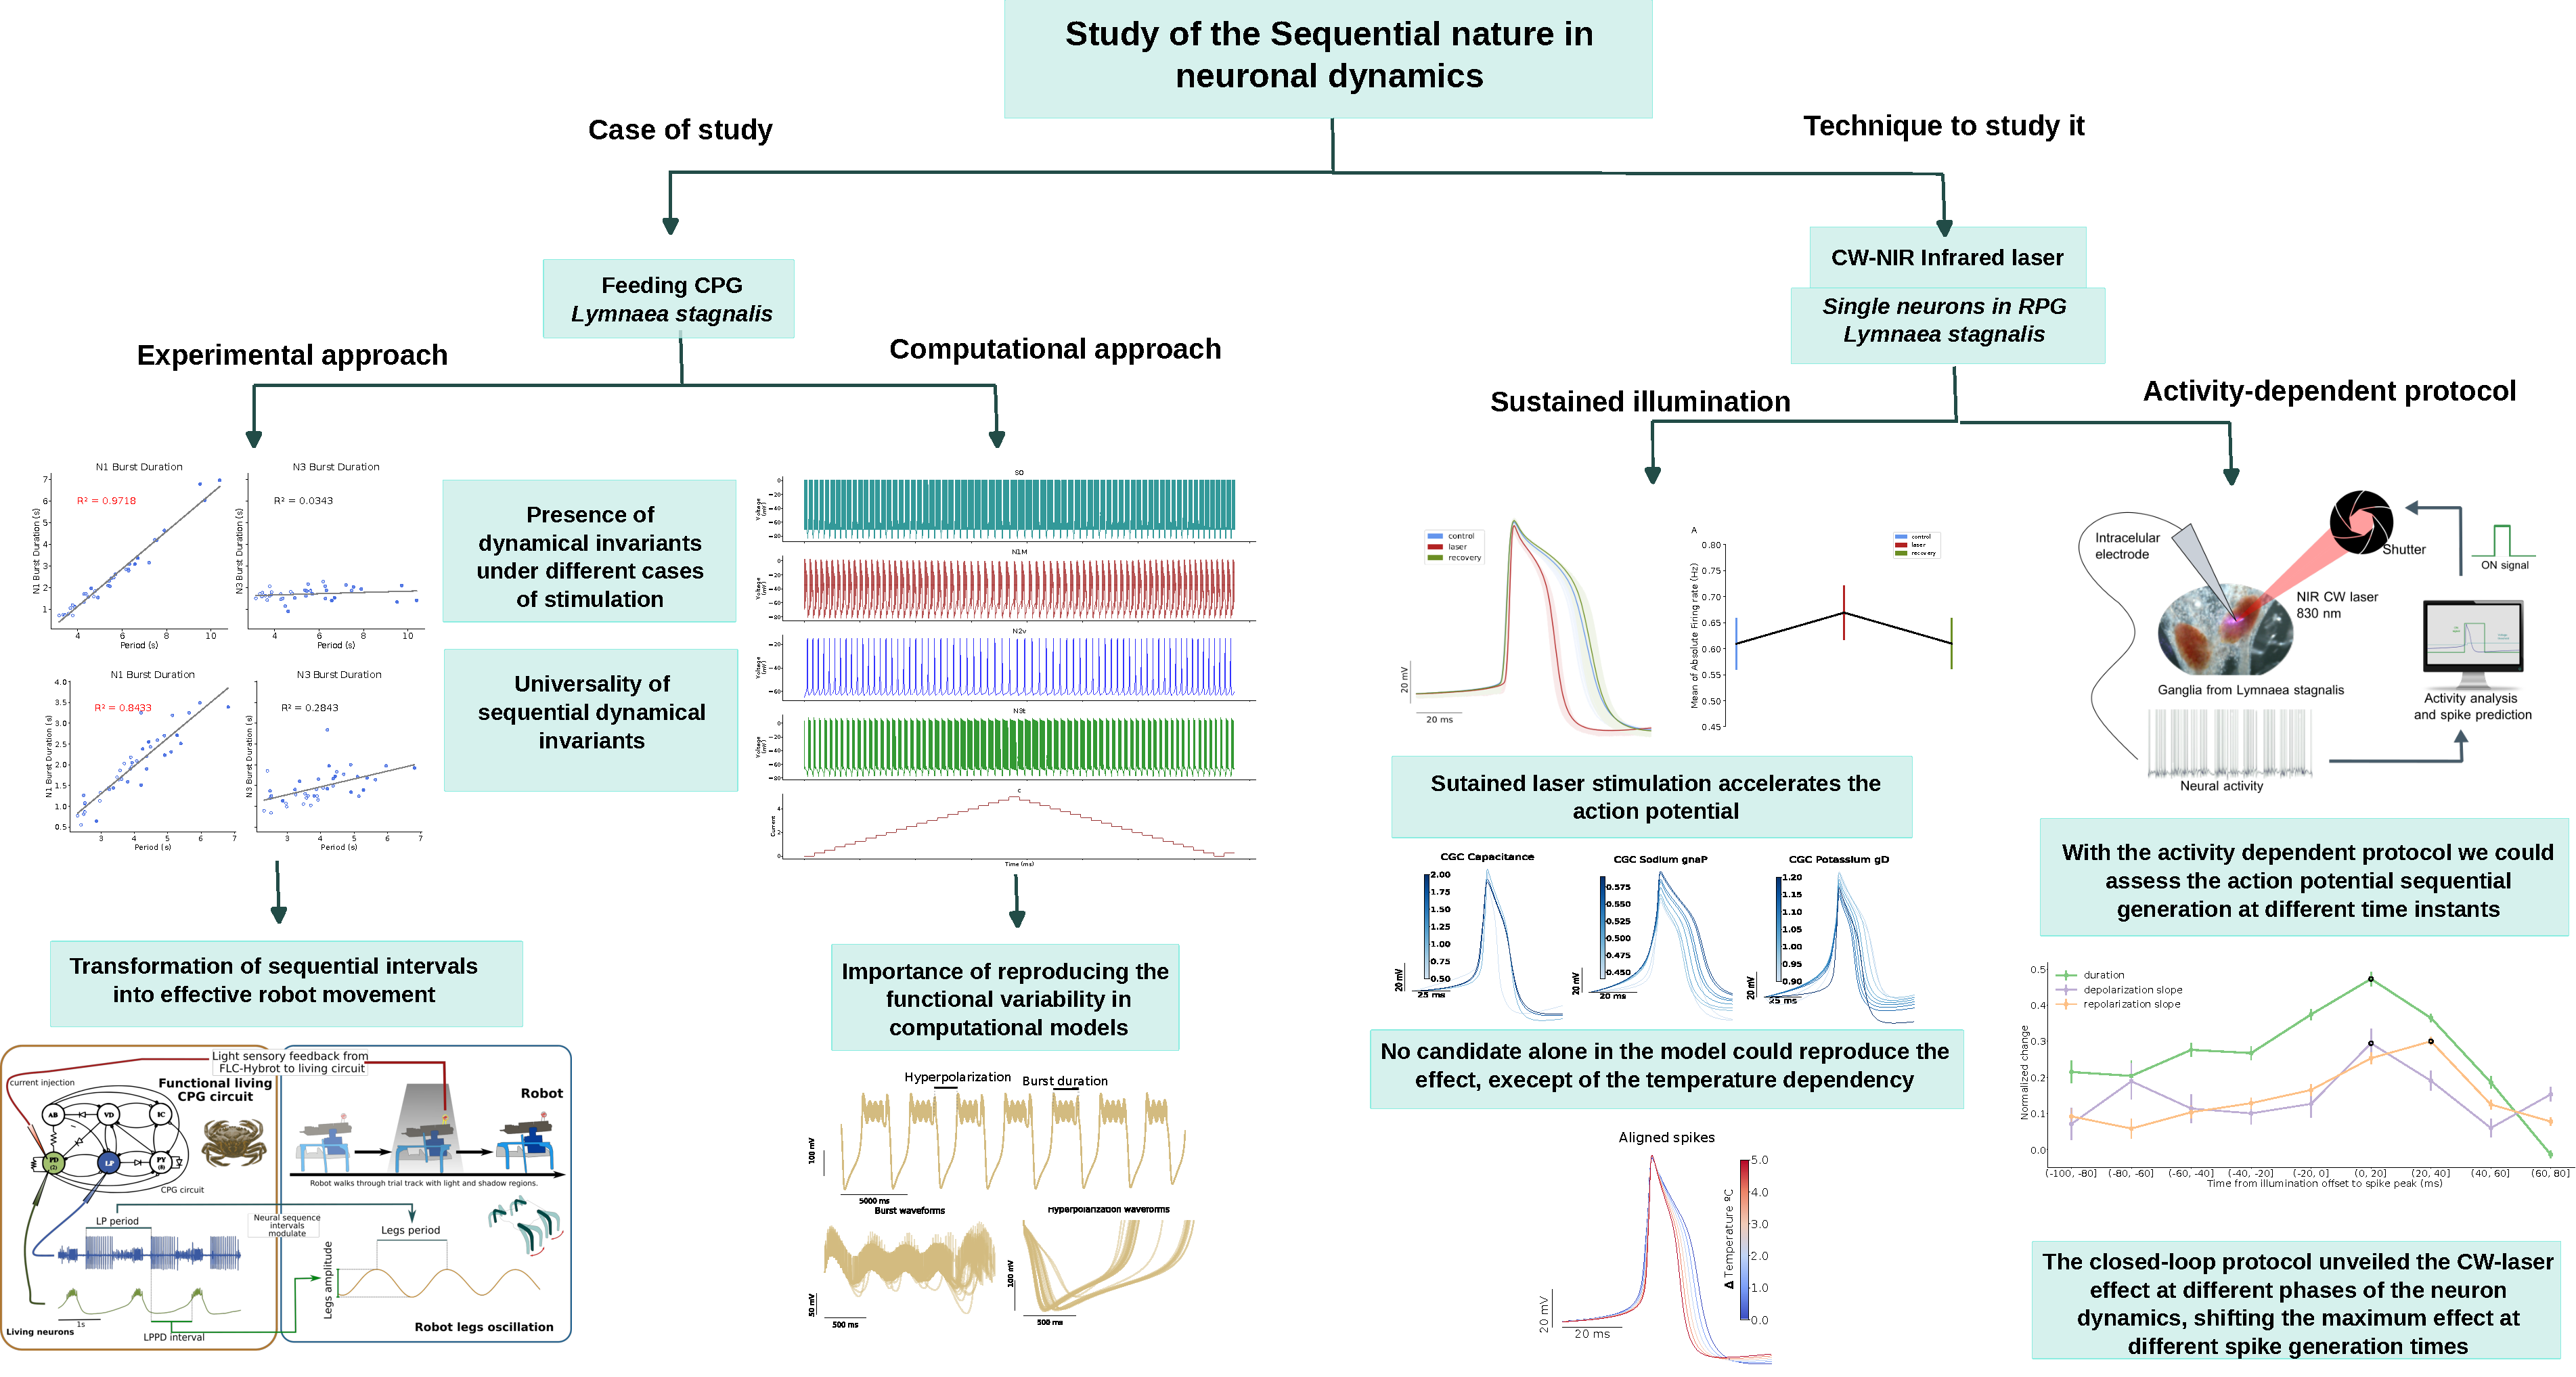
\includegraphics[width=0.9\textwidth]{img/panel discussion.pdf}
	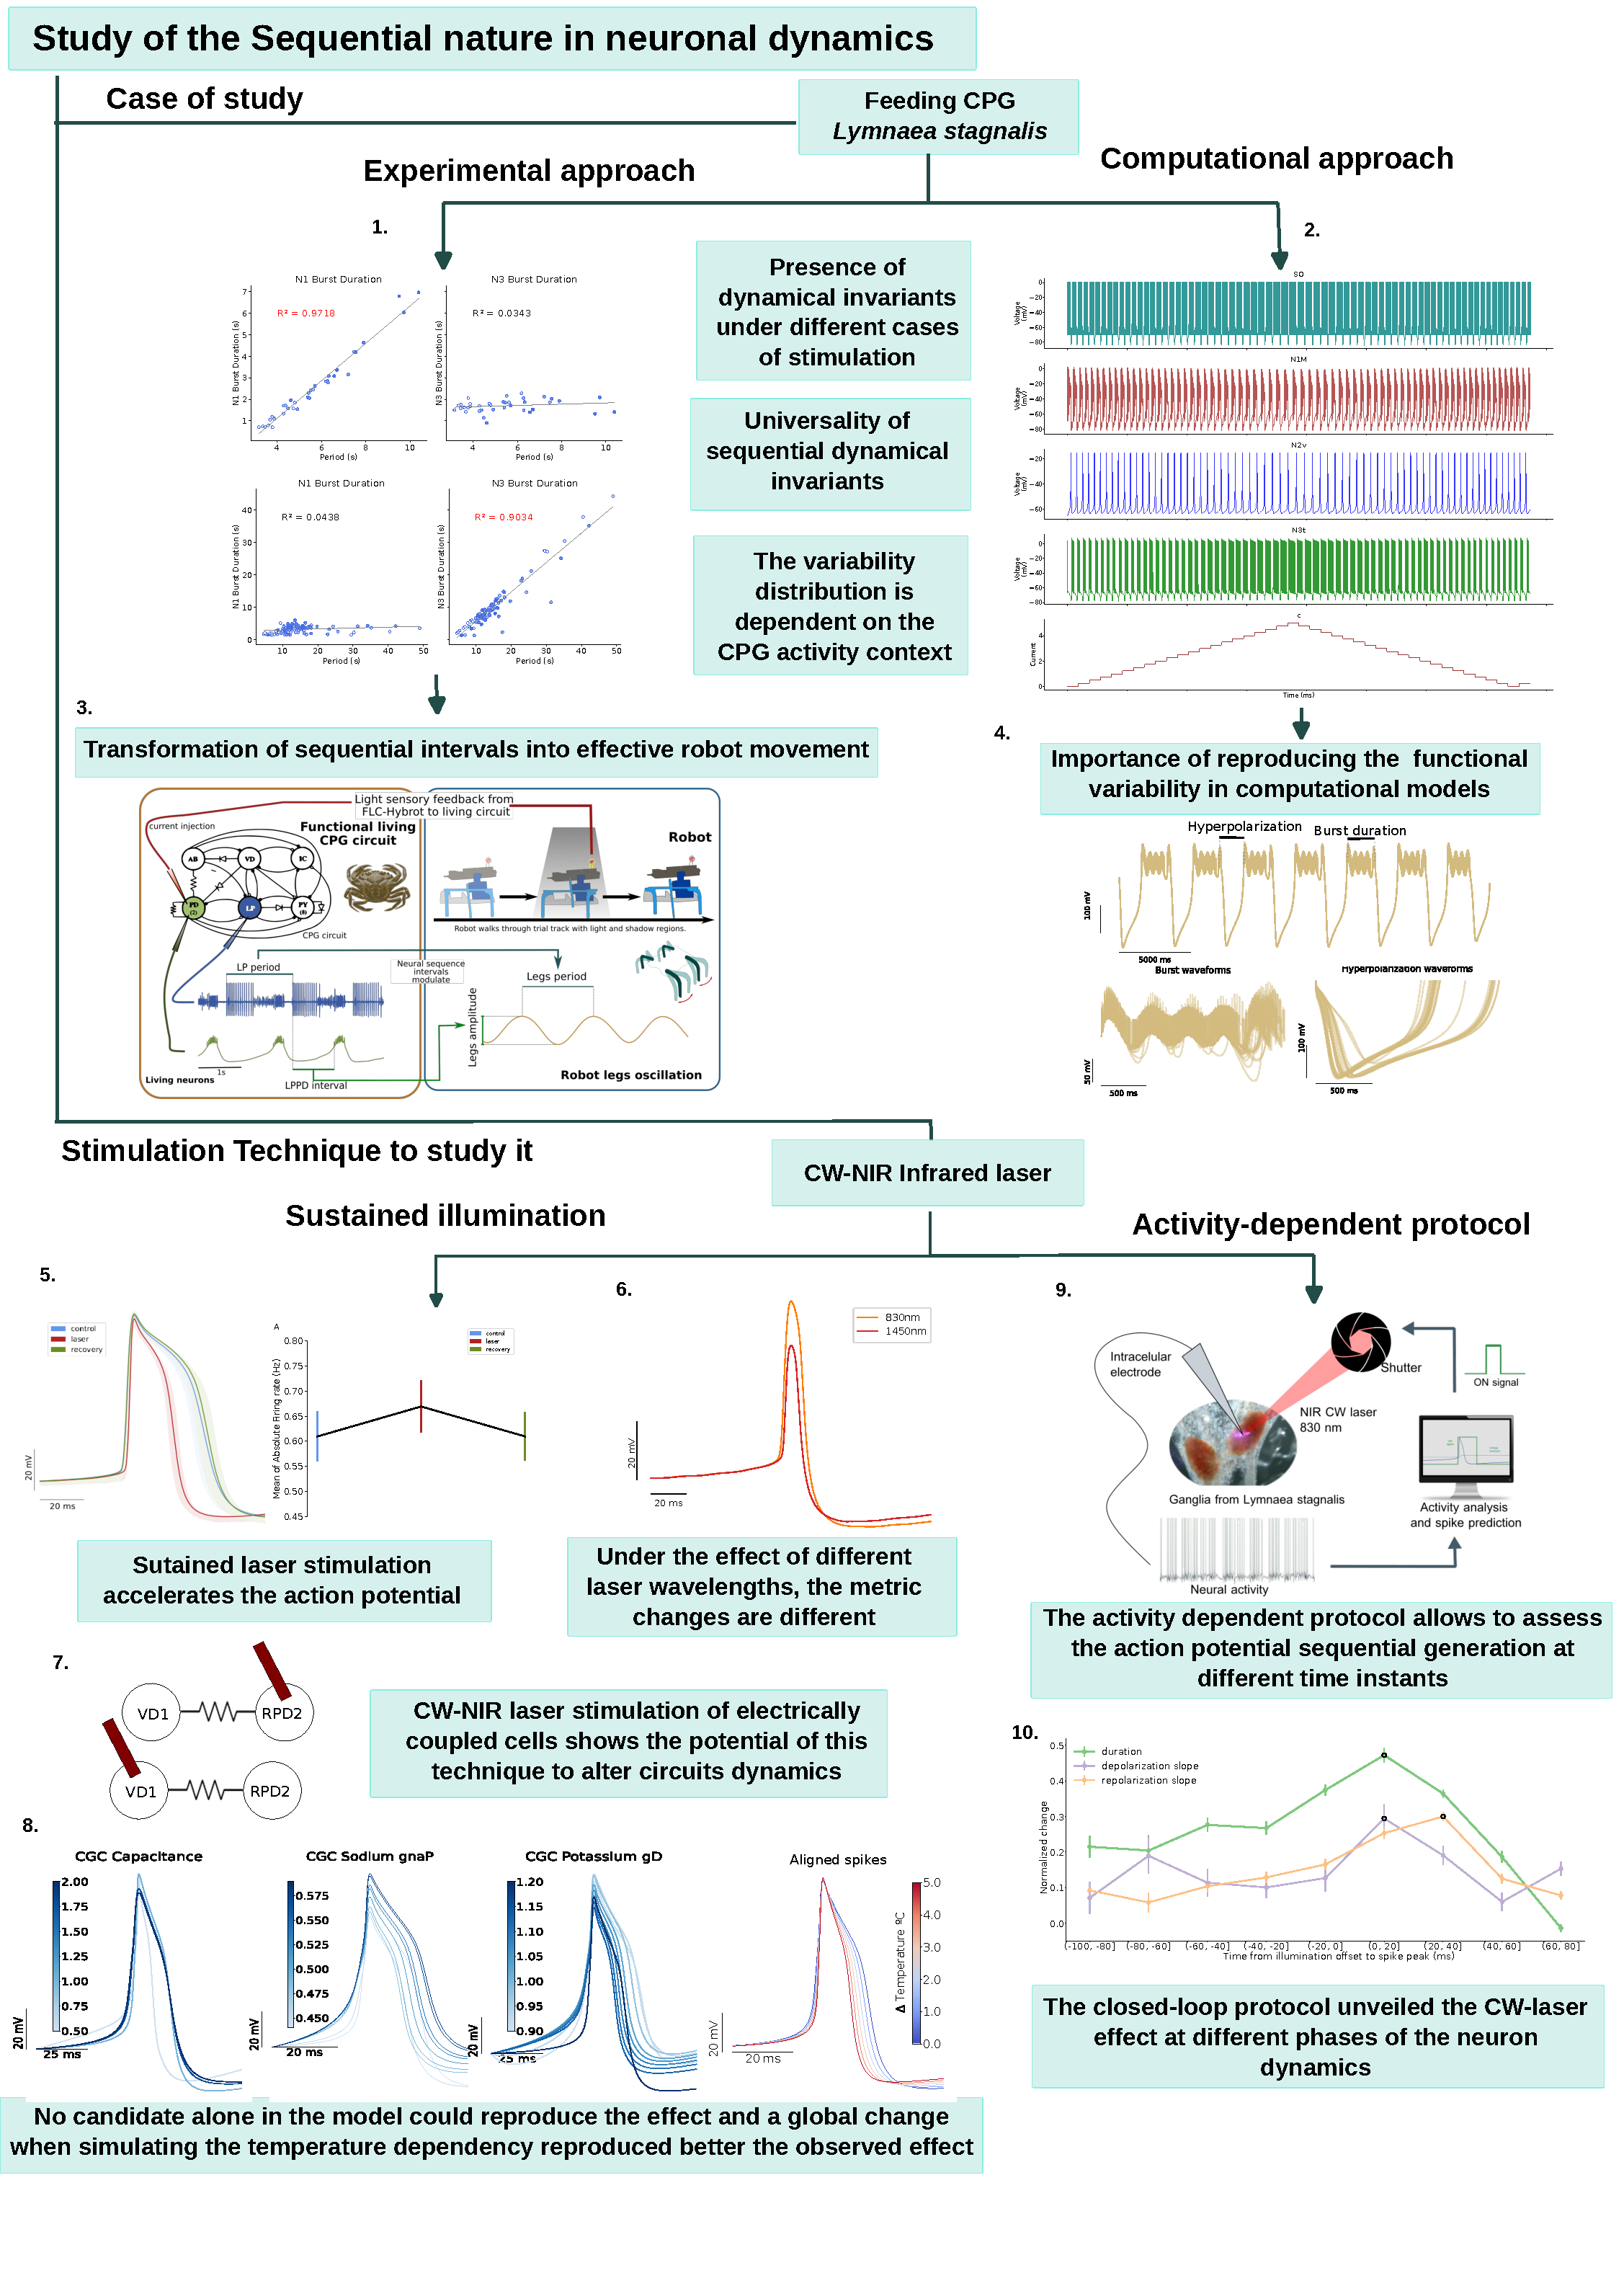
\includegraphics[width=0.75\textwidth]{img/panel_discussion_vertical_figures.pdf}
	\caption{Schematic summary of the results presented in this work. In the feeding CPG of \textit{Lymnaea stagnalis} we explored in experimental and computational data the presence of dynamical invariants (Secs. \ref{sec:experimental sussex} and \ref{c-invariants-model}), showing strong linear relations and associating this to the possible functional role of this indicator. The experimental results were complemented exploring the transformation of robot movement into effective robot movement maintaining strong linear relations (Sec. \ref{sec:robot}). We also showed the importance of reproducing the functional variability in computational models \ref{sec:model variability}. As a way to modulate neural dynamics we characterized the effect of the CW-NIR laser in single neurons in a sustained and activity dependent protocol. We showed the spike waveform is modified during the laser illumination, as well as the firing rate (Sec. \ref{sec:sustained effect}), and discussed the effect at different wavelengths (Sec. \ref{subsec:wavelengths}). We showed also preliminary results in the stimulation of a minimal circuit (Sec. \ref{subsec:electrical}). The computational model analysis revealed the combination of candidates to reproduce the effect and the importance of the temperature role (Sec. \ref{sec:laser models}). The activity-dependent protocol allowed to assess the action potential generation at different phases (Sec. \ref{sec:activity dependent}).}
	\label{fig:summary conlusions}
\end{figure}

	
During chapter 2 we analyzed the sequential dynamical invariants in a CPG circuit. The objective of that section was to proof the hypothesis presented in \cite{elices_robust_2019} that the strong linear relationships found between some intervals in the pyloric CPG of the \textit{Carcinus maenas} are not a specific feature of that particular CPG but a general rule for the effective motor activity generation in the CPG. Thus, the first result showed in \ref{c-invariants} is \textbf{(i) the universality of sequential dynamical invariants}, found also in the feeding CPG of \textit{Lymnaea stagnalis}. We proved this showing their presence not only in a detailed model of the circuit but also in experimental recordings of the CPG. In the model we saw how \textbf{(ii) it is possible to explore variability in the modeled circuit when induced by a ramp-current in specific neurons}. We explored the variability and the correlations between period and the different intervals in the cycle showing the sequential dynamical invariants, but that \textbf{(iii) the variability distribution and, consequently, the sequential dynamical invariants change as the neuron stimulated in the model simulation changes}. This highlights the importance of the circuit dynamics and the relation between the neurons so there is enough flexibility in the circuit to adapt to the variability cycle-by-cycle. We supported this results analyzing different recordings of from neurons in the buccal ganglion, that represented the circuit. We discussed in that chapter the difficulties defining the three phases of the feeding CPG in comparison with the pyloric CPG, where the neurons recorded in the circuit are inter-neurons. Thus, after identifying the three phases of the circuit based on different moto-neurons, we analyzed the variability and relations between intervals cycle-by-cycle for spontaneous activity cases and current stimulation driven activity in electrophysiological recordings. We showed the intervals variability and relations in three different examples of spontaneous activity and \textbf{(iv) found sequential dynamical invariants in the living spontaneous neural activity in the same intervals than the model.} We also analyzed different cases of stimulation, first SO driven stimulation, spontaneously and by induced stimulation, and reproduced the results in the model, \textbf{(v) showing a change in the variability distribution when the rhythm is modulated by SO.} From this premise that the rhythm is different as the source varies, we analyzed cases where the rhythm was modulated by CV1a neuron stimulation and by MLN nerve. In both cases, \textbf{(vi) the interval variability was shifted mainly between N1 and N3 phases under the different stimulation scenarios, although the tendency in CV1a is not as clear as under SO stimulation}.

In the study of the sequentiallity in CPGs we saw the importance of using effective tools to alter the spontaneous neural activity, in order to reproduce living mechanisms or achieve new behaviors. In chapter \ref{c-laser} \textbf{(i) we explored in detail the CW-NIR laser as a stimulation technique experimentally, theoretically and in activity-dependent protocols}. First, we show the effect of illuminating single cells and how \textbf{(ii) CW-NIR sustained illumination asymmetrically accelerates action potential dynamics and the spiking rate on single neurons.} We tested the sensitivity of the stimulation to the focus by \textbf{(iii) illuminating neurons electrically coupled, showing that the main modulation was in the directly illuminated neuron, slightly modifying the coupled neuron}. We also showed the preliminary results of the wavelength-effect relation, analyzing the effect in duration, amplitude and slopes with different laser wavelengths and powers, \textbf{(iv) showing a modulation of the amplitude as the laser wavelength increases that is not showed at low-wavelengths values.} This experimentally observed effect was dissected through model simulations, exploring the possible candidates: ionic channels and capacitance, in conductance-based models, with and without temperature dependence description, showing that \textbf{(v) no candidate alone could fully reproduce the observed modulation and that the global modulation through temperature description was the closest approximation to it.} Finally, \textbf{(vi)we presented a closed-loop protocol to alter the action potential at distinct sequential generation phases that can be generalized for distinct subjects and neurons}. With this stimulation protocol \textbf{(vii) we unveiled the CW-laser effect at different phases of the neuron dynamics, shifting the maximum effect at different spike generation times.} We also supported this results with \textbf{(viii) a model simulation, tuning some of the channels only at depolarization and repolarization phases, showing the enhancement of the effect as the focus time changes.}


Based on these experimental and theoretical results, we also presented in \ref{c-invariants} a study complementing both modeling and electrophysiological approaches. In the modeling side, \textbf{(vii) we analyzed the importance of variability in the study of neuronal dynamics and the limitation of most models reproducing the intrinsic functional variability of neurons}. We compared different examples of living and modeled neurons and their variability, \textbf{(viii) showing different models, their limitations and the best candidates to reproduce the functional variability by the description of the dynamics.} Regarding the experimental approach, we explored the possibility to transform the sequential intervals into effective robot movement. This is important in order to explain the functional meaning of this strong relationships we observed in specific intervals, that as we discussed is related to the context and the source of the rhythm. In this first prototype, \textbf{(ix) we analyzed and observed that it is possible to achieve an effective robot movement in a robot maintaining the strong linear relations}.

This study can have strong implications in neurorrehabilitation and brain progessing of motor activation, unveiling the key aspects of the relation between variability, robust sequentiality and flexibility that is shown in living systems, such as in CPGs. For this, it is necessary to expand the study of sequential variability in different animals but also to relate the sequential dynamical invariants to their role in the motor output, relating their activation to different contexts. In this direction, it is important first to improve the model simulations for both, circuit flexibility and relations and the description of chaotic dynamics of neural activity; and its expansion to more complex circuits and systems. The study of the time-interval restrictions in living circuits and the characteristics of it that produce and ensure the sequential dynamical invariants. And also the transformation of these restriction into effective visual examples such as the robot movement, reproducing the robustness of CPGs. This will be of high interest for neurotechnology and robotics design. 


The study of this novel technique might have strong implications for both research and clinical applications. Laser stimulation has been gaining ground in the field of optical stimulation, often studied as long-wavelength pulsed laser stimulation. It is important to validate different stimulation options such as the sustained continuous-wave here presented but also for activity-dependent stimulation. The protocol presented in this work might be enhanced with a larger precision, being able to stimulate at the nanoseconds scale. This will be relevant to extrapolate it to different systems, regardless of their neural activation time scale, but also to dissect precisely the channel activation dynamics. Furthermore, a in-deep characterization of the laser illumination and its safety range of activation will be of great importance for clinical applications. In this work, we showed a strong and reversible effect, that did not damage the neurons illuminated, which indicates the power used could be increased. A precise characterization of the power tolerated by the neurons would set the safety ranges of its application. Also, the preliminary study of the wavelength-effect relation showed that it is not only important the power but the laser wavelength in terms of the effect depicted, so the analysis  of the relation of the wavelength might expand this range of applications but also distinguish between other different mechanisms such as photo-electrical, photo-thermal, etc. Finally, as discussed in this work and laser neurotechnology literature, a photo-thermal effect is one of the main actuators behind the neuronal laser stimulation, however with the current tools and techniques it is not possible to have a detailed description of the change of temperature in the cell. In this line, although it is not included in this work, silver nanoparticles give a more precise estimation of the temperature change. 

% 7.2 Activity-dependent stimulation in the nanoseconds scale
% 7.3 Safety values of CW-NIR stimulation 
% 7.4 Temperature change in neurons estimation using silver nanoparticles


% Implicaciones de los resultados
% Trabajo futuro

